\begin{tcolorbox}[colback=red!5,colframe=DarkRed!40!black,title=Entry, Decent and Landing (EDL)]
Because of Curiosity’s large weight and size, it could not utilize landing procedures used for earlier rovers.
The new landing method is as unique as it is complicated.
The EDL-phase is therefore a spectacle popularly known as seven minutes of terror (referring to the time it takes after touching the atmosphere until it lands) \cite{CNN_7minterror}. 

The EDL sequence breaks down into four parts; guided entry, parachute descent, powered descent and the sky crane \cite{NASALanding}.

{\centering
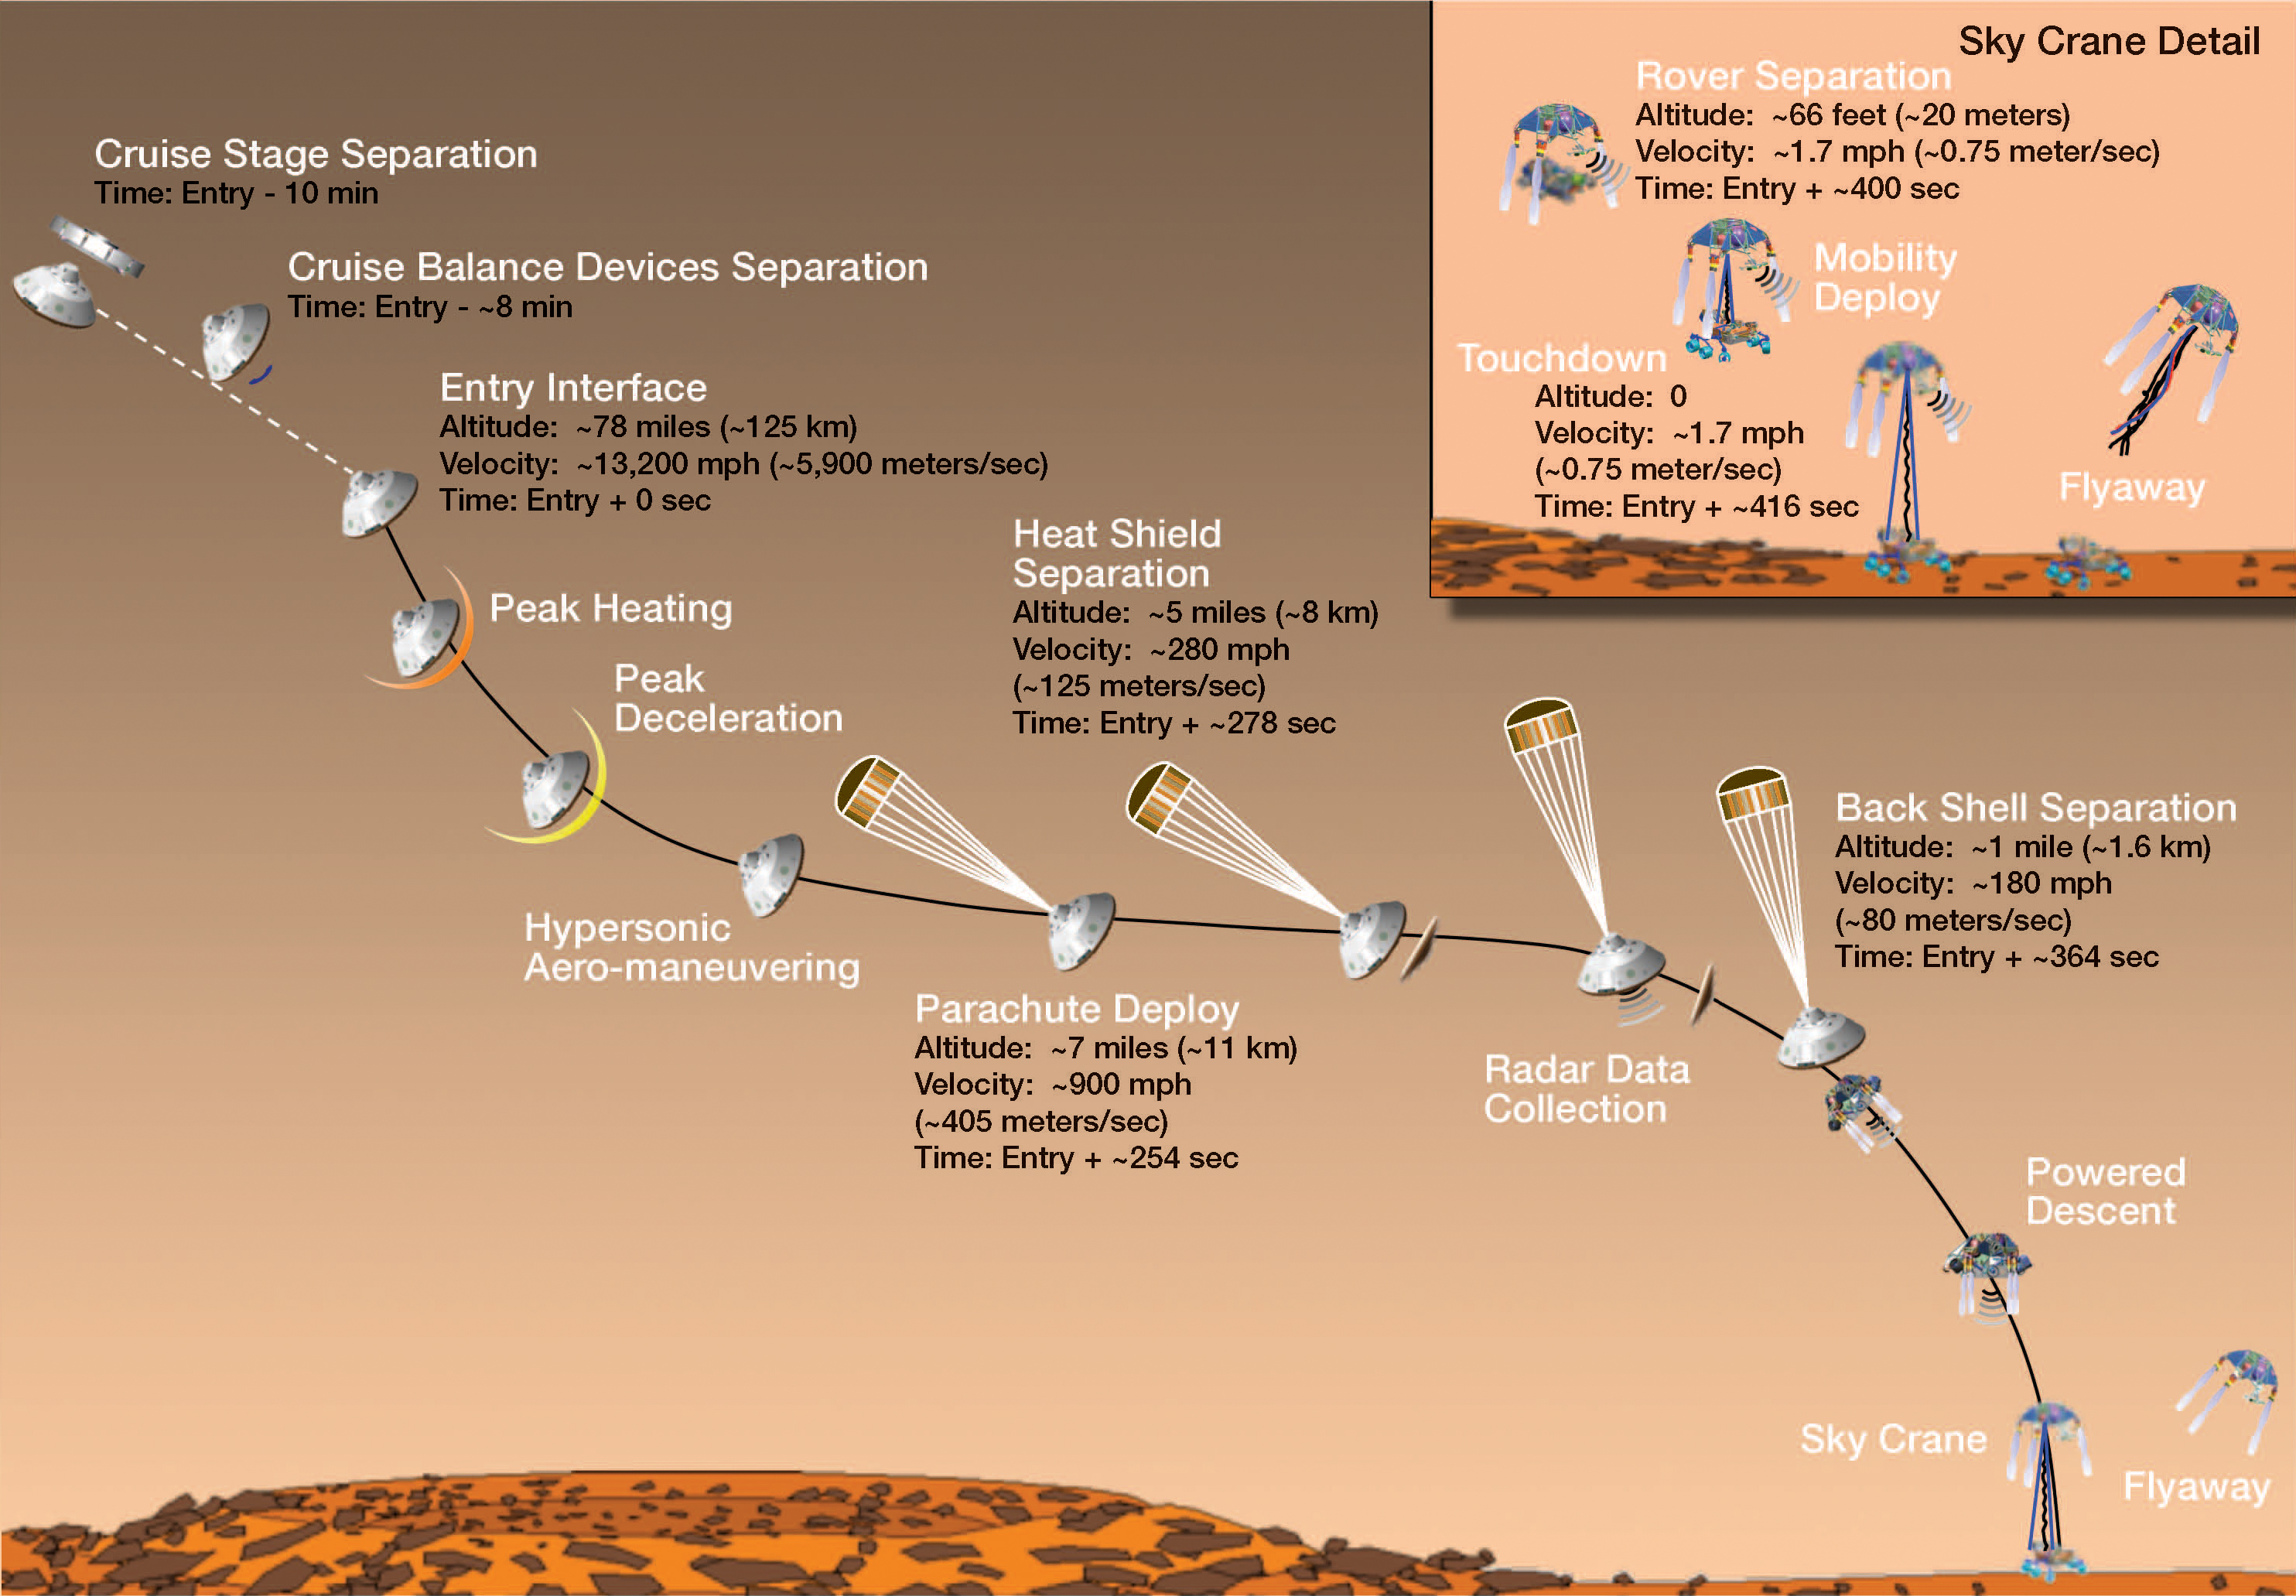
\includegraphics[width=\textwidth]{Curiosity_landing.jpg}
\par}

\textbf{Guided entry}
The spacecraft blasts into the Martian atmosphere at a whopping $21,240km/h$ crating so much aerodynamic drag the heat shield glows at $2,100\degree C$ \cite{NASA_youtube}.
The heat shield only manages to slow the spacecraft to a speed of $1,620km/h$ (because of the thin atmosphere) in which time the deceleration has created a maximum force equal to $16G$s \cite{HistoricLanding} \cite{NASALanding}.

\textbf{Parachute descent}
At this point, the largest and strongest supersonic parachute ever constructed for an extraterrestrial flight deploys. Capable of generating $24,500kg$ of drag force the spacecraft decelerate violently to a speed of $280km/h$ \cite{Parachute} \cite{NASALanding}.
Still way too fast for a landing there is only one solution; cut the rover loose.

\textbf{Powered descent}
The rover now in free fall, accelerates towards the surface at a rate of $3.7m/s^{2}$, fires eight rocket thrusters and reduces the speed to $14.5km/h$ while aiming for the landing site \cite{HistoricLanding} \cite{NASALanding}. 

\textbf{Sky Crane}
At an altitude of $27m$, the rover is detached from the descent stage and slowly lowered to the ground.
The descent speed is reduced to $2.7km/h$ and kept constant.
Then finally, on Aug. 5 2012, after a $5.6 million km$ \cite{CNNCuriosity} journey the rover touches down and pyrotechnically detaches itself from the descent stage.
The decent stage preforms a flyaway-maneuver crash-landing $150m$ away \cite{HistoricLanding} \cite{NASALanding}. 

7 minutes of terror completed.
\end{tcolorbox}